\newpage

\section{Crystal structure of Zircon/Zirconium(IV)silicate (ZrSiO4)}
\label{sec:ZrSiO4}

Using the Rietveld-wizard from Jana2006 we do the peak profilingand get the profile showed in figure \ref{fig:ZrSiO4Prof} and the parameters:

\begin{align}
    a=b=6.608\,\mathrm{\AA} \quad c=5.988\,\mathrm{\AA}
\end{align}

% \begin{center}
%     \begin{sidewaysfigure}
%     \centering
%     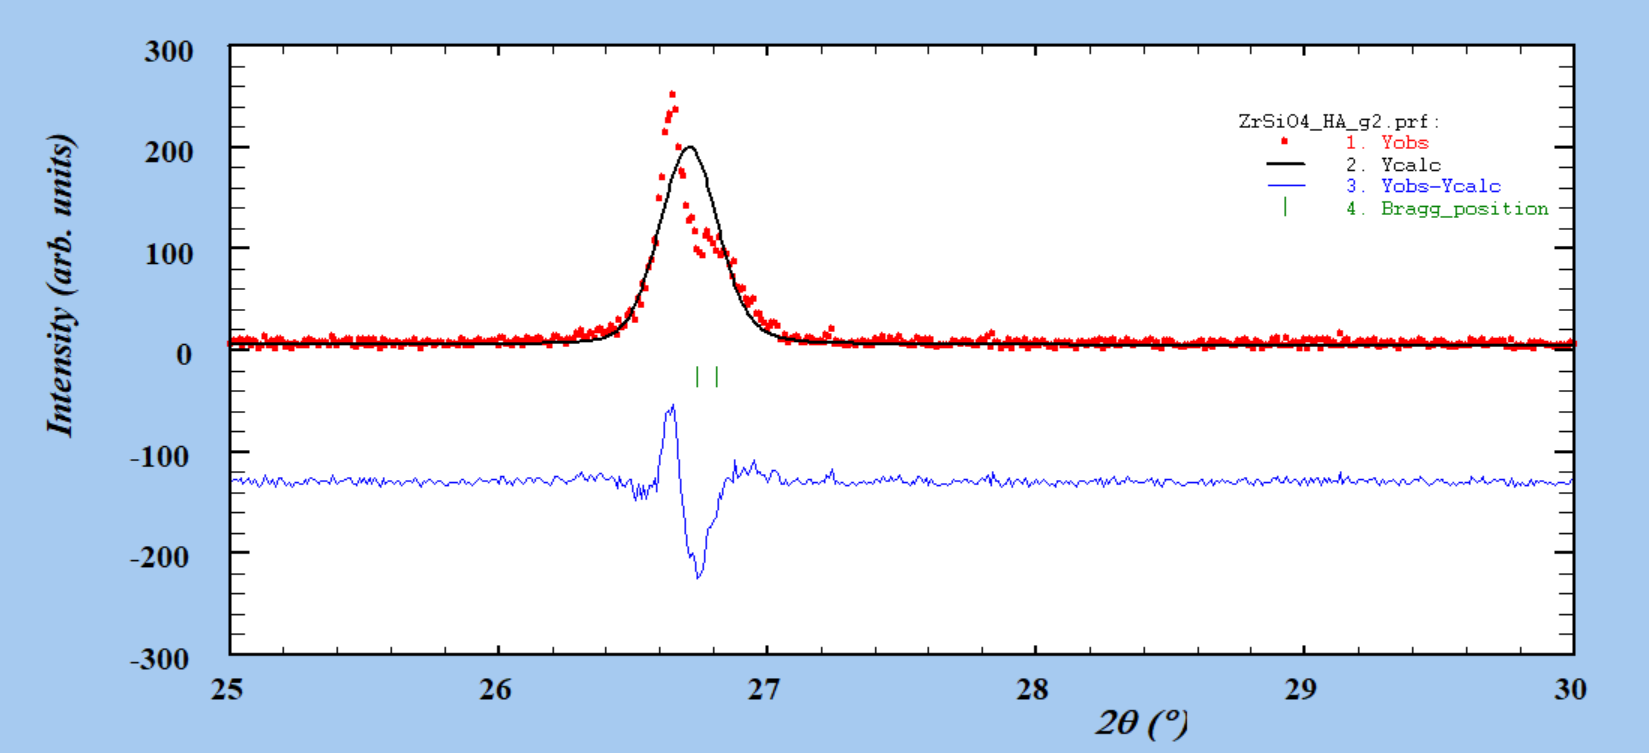
\includegraphics[width = 0.9\textheight]{Pictures/Evaluation/43/ZrSiO4DemoPeak.png}
%     \caption{
%         Due to the different distances between the $K\alpha$ lines and the two subpeaks of each peak, the profile could not be calculated exactly, but just as one pseudo-Voigt curve instead of a composition of two.
%     }
%     \label{fig:demoShitPeaks} 
%     \end{sidewaysfigure}
% \end{center}

\begin{center}
    \captionsetup{type = figure}
    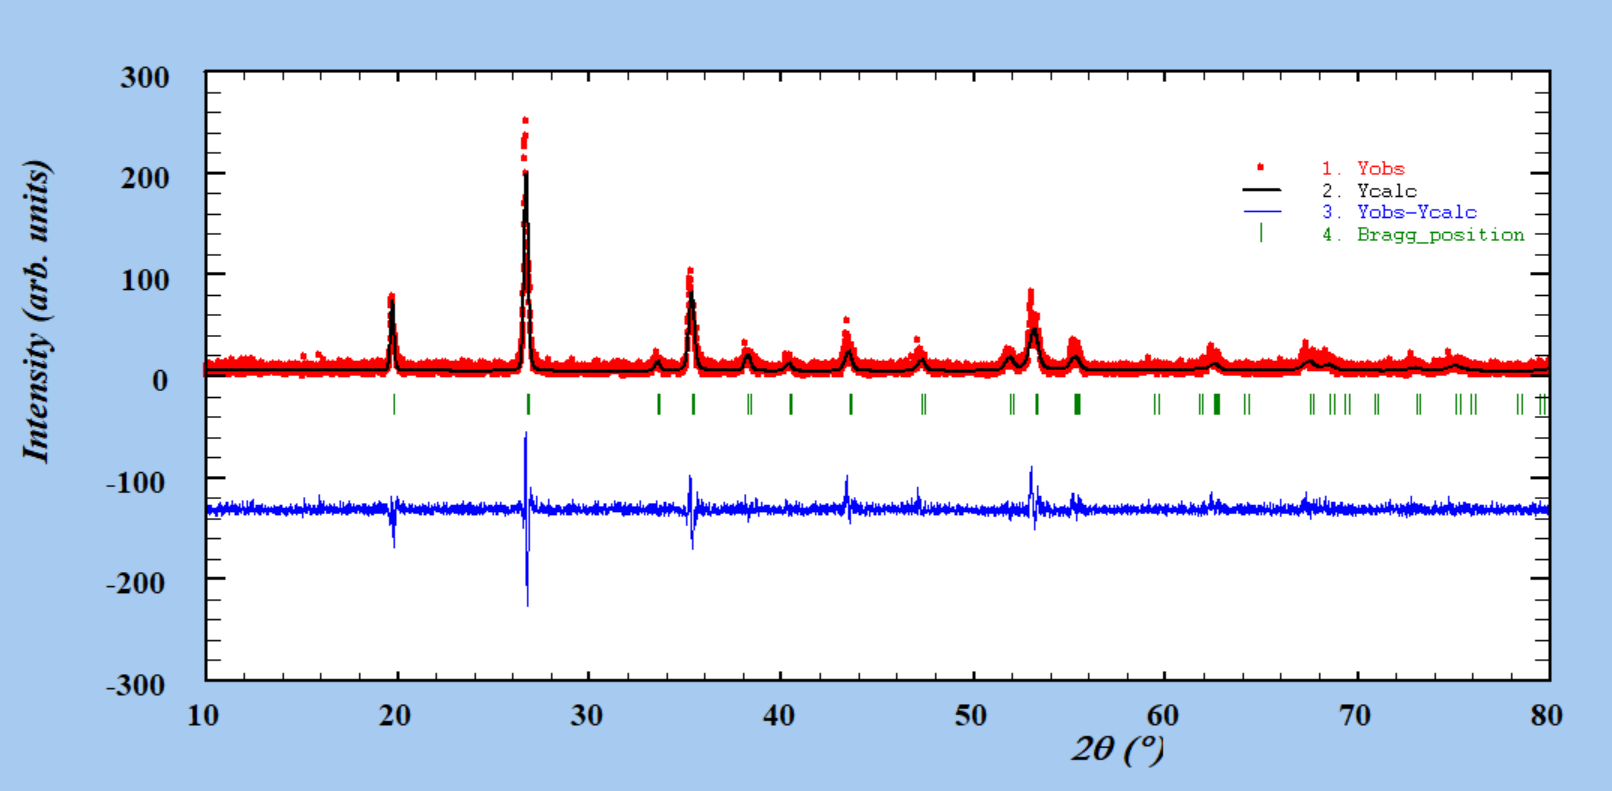
\includegraphics[width = 0.9\textwidth]{Pictures/Evaluation/43/ZrSiO4DataAll.png}
    \captionof{figure}{Resulting profile}
    \label{fig:ZrSiO4Prof}
\end{center}
Te difference plot shows some peaks,  which are due to inaccuracies.

Furthermore, the structure shown in figure \ref{fig:ZrSiO4Struct} were generated via Jana2006.


\begin{center}
    \captionsetup{type = figure}
    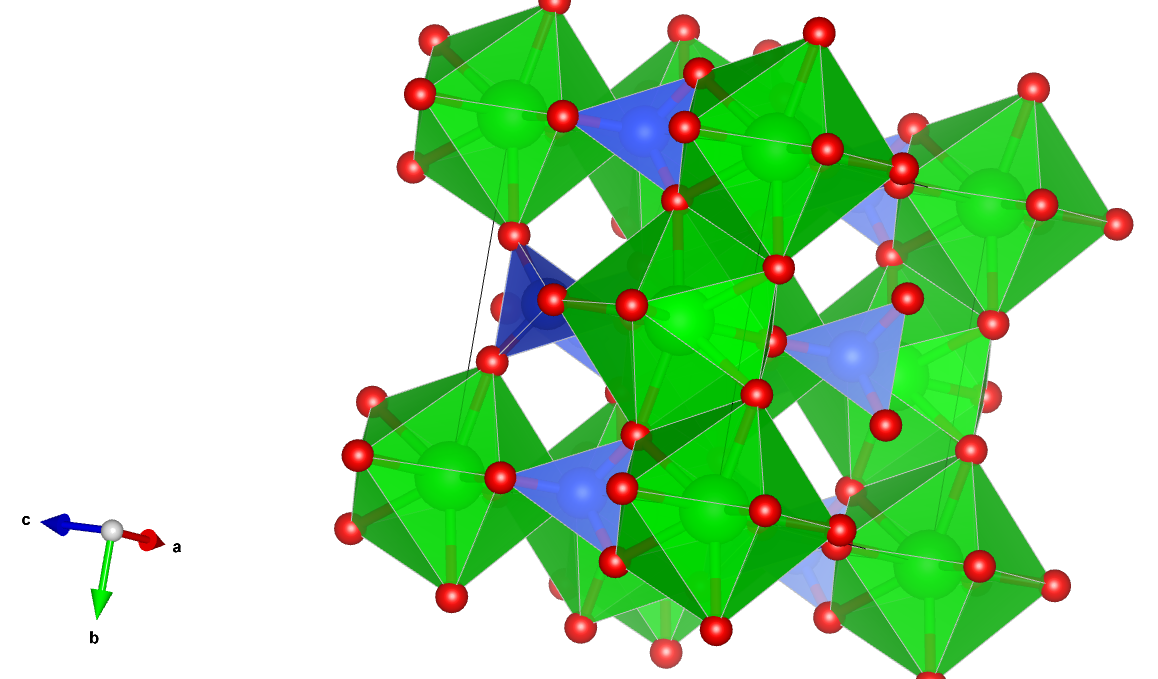
\includegraphics[width = 0.7\textwidth]{Pictures/Evaluation/43/ZrSiO4StructurePolyhedral.png}
    \captionof{figure}{
        Structure model in polyhedral style. ZrO\textsubscript{8} trigondodecahedra in green and SiO\textsubscript{4} tetrahedra in blue. 
    }
    \label{fig:ZrSiO4Struct}
\end{center}